% REMEMBER: You must not plagiarise anything in your report. Be extremely careful.
\documentclass{l4proj}

    
%==============================================================================
% Put any additional packages here
% You can add any packages you want, as long as it does not alter
% the overall format (e.g. don't change the margins or the reference style).
%
\usepackage{pdfpages} % if you want to include a PDF for an ethics checklist, for example
%
%

\begin{document}

%==============================================================================
%% METADATA
\title{Programming Language Translation} % change this to your title
\author{Scott Johnston}
\date{September 14, 2018}

\maketitle

%==============================================================================
%% ABSTRACT
\begin{abstract}
With the number of different programming languages available on the market today, all offering different advantages, a programming language translator which would allow code to be converted from one language to another effectively is desirable. For this Honours project, I worked to develop a translation tool using the ANTLR framework, that would allow code in Java to be converted into Python.
Despite their prevalence of these languages in modern programming, the development of this tool is relatively unique. The tool that shall be discussed will allow for code between the two languages to be translated with ease and with decent accuracy, and shows massive potential to be powerful in the future, which will also be discussed in this thesis.


    Every abstract follows a similar pattern. Motivate; set aims; describe work; explain results.
    \vskip 0.5em
    ``XYZ is bad. This project investigated ABC to determine if it was better. 
    ABC used XXX and YYY to implement ZZZ. This is particularly interesting as XXX and YYY have
    never been used together. It was found that  
    ABC was 20\% better than XYZ, though it caused rabies in half of subjects.''
\end{abstract}

%==============================================================================
%% ACKNOWLEDGEMENTS
\chapter*{Acknowledgements}
I would like to thank my supervisor Derek Somerville for his guidance and support over the past year. I really valued the creativity Derek provided, as well as helping me through the unprecedented difficulties provided by the COVID-19 pandemic.

% Enter any acknowledgements here. This is optional; you may leave this blank if you wish,
% or remove the entire chapter
%
% We give thanks to the Gods of LaTeX, who in their eternal graciousness, 
% have granted that this document may compile without errors or overfull hboxes.
%

%==============================================================================

% EDUCATION REUSE CONSENT FORM
% If you consent to your project being shown to future students for educational purposes
% then insert your name and the date below to  sign the education use form that appears in the front of the document. 
% You must explicitly give consent if you wish to do so.
% If you sign, your project may be included in the Hall of Fame if it scores particularly highly.
%
% Please note that you are under no obligation to sign 
% this declaration, but doing so would help future students.
%
\def\consentname {Scott Johnston} % your full name
\def\consentdate {16 February 2021} % the date you agree
%
\educationalconsent


%==============================================================================
\tableofcontents

%==============================================================================
%% Notes on formatting
%==============================================================================
% The first page, abstract and table of contents are numbered using Roman numerals and are not
% included in the page count. 
%
% From now on pages are numbered
% using Arabic numerals. Therefore, immediately after the first call to \chapter we need the call
% \pagenumbering{arabic} and this should be called once only in the document. 
%
%
% The first Chapter should then be on page 1. 

% PAGE LIMITS
% You are allowed 40 pages for a 40 credit project and 30 pages for a 
% 20 credit report. 
% This includes everything numbered in Arabic numerals (excluding front matter) up
% to but *excluding the appendices and bibliography*.
%
% FORMATTING
% You must not alter text size (it is currently 10pt) or alter margins or spacing.
% Do not alter the bibliography style. 
%
%==================================================================================================================================
%
% IMPORTANT
% The chapter headings and structure here are **suggestions**. You don't have to follow this model if
% it doesn't fit your project. Every project should have an introduction and conclusion,
% however.  If in doubt, your supervisor can give you specific guidance; their view takes precedence over
% the structure suggested here.
%
%==================================================================================================================================
\chapter{Introduction}

% reset page numbering. Don't remove this!
\pagenumbering{arabic} 

% You can use \todo{} to mark text that needs to be fixed. Anything inside will appear as highlighted 
% text in the final copy, and you will also get warnings when you compile (so you don't
% forget to take them out!)

\section{Background}
\subsection{Programming Language Translation}
 Program conversion process has been placed  among  the  top  10  challenges  in  the  programming  world  (Terekhov, A. A., & Verhoef, C., (2000) "The realities of language conversions". IEEE  Software,  vol. 17, no. 6, pp. 111-124.) Whilst there exists many tools online to try such a thing, it is an area of research which is yet to be cracked. The motivation for such a tool is clearly there however, due to the amount of research that has been done into conversion tools. There has also been a number of discoveries made into how best to translate code, with a lot of experts agreeing on an intermediate layer between the two languages. This concept is fully explored by Coco, Osman and Osman in their paper "JPT: A Simple Java-Python Translator". This involved the use of an XML middle-layer to try and translate the basic principles of programming languages from Java into Python. As things stand, there are a multitude of translators on the market to and from the most popular programming languages about, however the process of re-engineering certain codes due to the uniqueness of different languages semantics and syntax, has meant that sophisticated code is difficult to convert. 
 
\subsection{Java2Python}
Java2Python is the most recognisable tool that is available, and holds similar abilities to the tool that this project intends to produce. Java2Python uses ANTLR to create an abstract syntax tree from the source code (java file) and walks the tree's nodes, converting each node to it's Python equivalent. This is a similar approach taken in this project, but with some key differences that will be discussed late in the design chapter. Java2Python exists in the Python Package Index (PyPi), meaning it has been recognised by Python themselves, as a useful package. It is described on their website as a tool to "imperfectly translate Java source code to Python source code". This imperfection will also be discussed later in the background chapter of this paper, including the fact it is outdated, it's clear limitations, and it's verbose nature causing confusion.
\subsection{ANTLR and StringTemplate}
The Programming Language translator is built primarily using the ANTLR framework along with stringTemplate.

\subsubsection{ANTLR}

ANTLR stands for "Another Tool for Language Recognition". The framework uses a user-generated grammar file to generate a parser which can then be used for reading, processing, executing, or in this case, translating structured text files. ANTLR was built in Java however has been developed to allow users to use this tool with any type of target language (for example, the Java2Python application built the backend in Python). ANTLR is widely used in academia and industry to build all sorts of tools, frameworks and languages, including the Twitter Search, for query parsing. This shows the power and reach the ANTLR tool has.

\subsubsection{StringTemplate}
StringTemplate is a java template engine which can be used to output source code. A template engine is a code generator that emits text using templates, which are essentially just text documents with spaces for attributes to be added. These attributes will be found via the parser generator (in this case ANTLR) which will direct the attributes to the correct template.
\subsubsection{Combining ANTLR and StringTemplate}
These two softwares collaborated nicely due to stringTemplate powering ANTLR, and justification for how and why they were used can be found in the design and implementation section of this thesis.
To briefly explain it however, there is a Java grammar that exists in ANTLR, which is then parsed, essentially identifying nodes of attributes. These attributes are then fed into the Python StringTemplate to output Python source code. This approach was primarily inspired from the following document, explaining how the two combined to give a very simple translator:
https://theantlrguy.atlassian.net/wiki/spaces/ST/pages/1409118/Language+Translation+Using+ANTLR+and+StringTemplate

\subsection{Impact of COVID-19}
The 2020-21 academic year has been gravely impacted by the ongoing global pandemic. This had an indirect yet significant affect on this honours project. Face-to-face communication has been extremely restricted throughout the year, meaning that meetings with supervisors were limited to online calls via microsoft teams, which many would argue is harder to be engaged with.

On top of this the pandemic situation was anxiety inducing, which many recent studies, including "Onboarding during Covid-19: Create Structure, Connect People and Continue Adapting" by Charles Scott, have proven has lead to students struggling with motivation towards their studies. The university did however regularly update students with advice on coping throughout these troubling times.

Ultimately, this project was not majorly influenced by the global pandemic, as the software tool could be built and evaluated without external tools supplied by the university. In general however, opportunities were restricted, making the likes of interviews very difficult to be carried out.

\section{Problem Space}
\subsection{Java and Python}

The decision to focus on a translator between Java and Python ultimately came from the fact that these are the two most prevalent programming languages in the Computing Science course at University of Glasgow. However there is strong justification for this language choice due to their relevance.

\subsubsection{Python}
Python is a highly popular language for a number of reasons, most notably it is easy to read and write, it is an interpreted language, it is dynamically typed, and it possesses a rich base library and garbage collection feature. (https://python.land/python-tutorial/what-is-python) A paper by Fangohr detailed a comparison carried out between C, MATLAB and Python as teaching languages in engineering. This paper heavily supports that python has an easy-to-use syntax and highlights that python is here to stay in industry, due to it's intuitive nature. A paper titled "An Empirical Comparison of Seven Programming Languages" also mapped the advantages of python performance-wise using empirical data, as it performed amongst the best when put up against 6 other well known programming languages. This evidence of both strong performance and syntactical-ease are enough to justify the importance of Python, thus the decision to use it as the target language for the programming language translator was clear.


\subsubsection{Java}
According to Oracle, 3 billion devices run on Java. This proves it's popularity, probably due to it's many advantageous factors. One major factor being the embrace of object-oriented programming (OOP) in contrast to the procedural programming approach associated with a lot of other languages. Other advantages include Java's platform-independency, it's support for a plethora of libraries being appealing to enterprise computing and Java's support for common programming key issues such as multi-threading and automatic memory management. 

\subsubsection{Translation from Java to Python}
Object-Oriented Programming is at the core of all Java programs, which is untrue for Python, despite having OOP capabilities. Java is restrictive and complex to design in comparison to the intuitive nature of python. Java is also statically typed (meaning that a variable's type must be defined), whilst Python is dynamically typed.

Evidently both Python and Java are powerful and popular for a reason, justifying their place as two of the top languages in the programming world. The differences that have also been highlighted are areas which will make the translation process interesting and justifies that there is enough of a difference between the two languages to make a translation tool worthwhile.

Further justification could come from the legal battle currently ongoing between Oracle (owners of Java) and Google. Oracle want a share of the money Google have made from Android, somewhere in the region of a billion US dollars, because of the several Java APIs that have been re-implemented into Android. This battle has been ongoing for 10 years, with both sides of the debate spending several millions of dollars to fight their case. If Oracle were to win this legal battle, it will likely deter businesses from using Java in the future and they may rush to change the programming language they operate in completely. Python would be one of the obvious alternatives due to it's recent popularity.

\section{Motivation}
Whilst it is not believed that Python will replace Java, given the benefit of some python features highlighted in section 1.2, there is definitely an existing argument as to why people may choose to code in python. Aside from this, Python is also closely related to newly emerging fields in computing science such as the Internet of Things (IoT).

In a 2019 article it was suggested by TIOBE that Python could overtake both Java and C to become the most popular programming language in the world. This was due to the "software engineering boom" which attracted newcomers to programming. To understand a simple program such as "hello world" a java user must understand classes, static methods and packages, whilst a C user is required to understand explicit memory management. A Python user however, simply must understand one single line.
The article goes on to explain how Python is widely regarded the first programming language taught to university students, however not only due to it's simple high-level syntax. It is due to Python being the number one language in a number of different computing domains such as statistical, AI programming, scripting, system tests, web programming and scientific computing.

Figure \ref{fig:index} shows the TIOBE Programming Community index from February 2021. This index is used as indicator of the popularity of programming languages. The ratings use popular search engines to calculate the ratings, and is based on the number of skilled engineers world-wide, courses and third-party vendors. The graphic clearly indicates the rise of Python and relative fall from Java (Despite still being number 2 in the overall rankings). This evidence benefits what was stated in the 2019 article about Python's rise in the next few years.

This evidence combined makes Python a strong candidate to soon dominate the software market. This in turn could create the shift in many different industries from their current software (in a lot of cases a Java software) to one operated in Python. This could become a tedious job, and rewriting software in a new language from scratch would be both time consuming and expensive. Therefore, a mechanism that converts Java (a vastly popular programming language that is starting to wane) to Python (a language which is massively increasing in popularity) relatively accurately and automatically, could be imperative in the software development world in the near future.

\begin{figure}[htb]
    \centering
    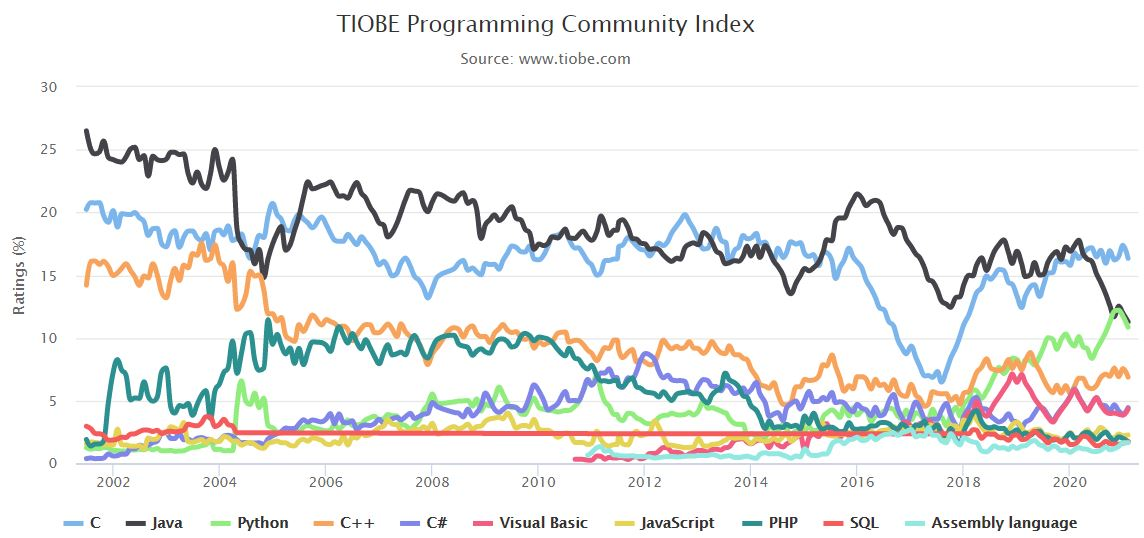
\includegraphics[width=1\linewidth]{images/Programming Community Index.JPG}
        \caption{TIOBE Programming Community Index from February 2021. Focus should be on the green line showing Python's strong growth between 2018-present. 
    }
    \label{fig:index} 
\end{figure}

A paper titles "Python - The Fastest Growing Programming Language" is further evidence for a move to Python. The paper details the many benefits of Python, which have roughly been covered in this paper already. It then goes on to discuss how being able to code in Python is now a more in-demand skill than ever, stating that in terms of search volume, learning Python is the \#1 search when compared to other programming languages. On top of this, Python is an open-source project, with a moderate update cycle, with new versions coming out about once a year. This allows Python to stay relevant which cannot be said about certain other popular languages, with Java updates less regular and significant, and C updates being non-existent.

\section{Research Questions}
As briefly summarised in section 1.3, the overall goal was to try and create a tool which would convert a program written in Java to Python, without compromising accuracy or code quality. Aside from this overall goal, objectives were set out which were altered as the project went on to fit with what had been achieved. 

Upon some background research which shall be touched upon in Section 2,  Program conversion process has been placed  among  the  top  10  challenges  in  the  programming  world (https://ieeexplore.ieee.org/stamp/stamp.jsp?tp=&arnumber=895180), and the comparison of programming language conversion to "turning a sausage into a pig" from the same paper, shows that this was not going to be a straightforward task. A fully functioning translator with 100\% accuracy was not achievable given the time frame and skill level, and some would even argue impossible to ever have such a powerful translator. An example of why this is impossible could be a package with certain capabilities existing in Java but not in Python.

Nevertheless, the following objectives were decided upon:
\begin{itemize}
    \item
    1) Ensure simple/common coding paradigms can be translated (explanation below)
    \item
    2) Ensure the code is expandable for future work.
    \item
    3) Ensure through evaluation that translator is at least as good as what is on the market
    \item
    4) Keep translations as simple as possible 
\end{itemize}

For the sake of clarity here is a more thorough description of each objective.

\subsection{Objective #1}
Consideration was taken into what is the most useful and common coding patterns used in Java that should be implemented into the translator. Given my own coding experience accompanied by W3Schools.com (which offers tutorials for beginners), these were selected as follows:

Conditional statements in the form of if/else/ else if as well as logical conditions using mathematical symbols (e.g 'a>'b, 'a<b', 'a==b').

Switch statements, which are a form of conditional statement to select a block of code that executes if a case is met (switch/case/default)

While loops, and do/while loops where a block of code will be executed as long as a specified condition is reached.

For loops, where the number of times code will be looped is specified, rather than a condition waiting to be met. Also for-each loops can be used when looping through elements in a list-type structure such as an array.

Also included in this objective, would be converting the OOP structure required in Java into Python, Which meant creating classes and methods in the translation. This is not only good coding practice, but meant the code could be easily compared due to the shape remaining similar.

The ANTLR grammar file used for translation was also imperative in finding what areas of the Java programming language to focus on. This file will be discussed later in the design phase of this thesis.

\subsection{Objective #2}
This objective was actually decided upon during background research when looking for similar software tools that had been built. Whilst there was some helpful research, a lot of the tools were difficult to use any source code from, due to their unclear structure. 
This meant that even if my translator was just to be a "proof of concept", the way in which it should be built is so that it is extendable, such that the 'future work' set out in this thesis could possibly be built using the framework I have managed to design so far.


\subsection{Objective #3}
For this objective, there was a few translator tools on the market that did a similar thing to what this was intended to do, and decided that for this to be a success, the evaluator should perform at least as well as what is currently on the market. This meant testing my tool with the java2python test folder that can be found at https://github.com/natural/java2python/tree/master/test and I intended for my evaluation to be a success if my tool converted all these tests with accuracy and perhaps could improve upon this tool through a comparison. This objective will be discussed further in the evaluation phase of this thesis.

\subsection{Objective #4}
For Objective \textbf{\#4}, I did not want to make translation overly complicated. A philosophy adopted with this tool from early on was that if the translation can be simplified, it has not been fully successful. This idea came from my evaluation of other translation systems, as I felt some conversions, whilst able to compile and run successfully, the translation looked over complicated and thus, may be too indecipherable and very difficult to maintain and add features to.

\section{Contributions}

\subsection{What has been Learnt}

Programming translation is a topic that on the surface seems relatively straight forward. This project taught the true hardship behind creating a powerful programming language converter, and where issues can occur. It was also an eye opener to some of the great frameworks available and the research into the project which made the future of programming language translation seem somewhat more reachable. It also taugh a lot about how a translator should be evaluated and tested, and at what point the tool can be considered effective.

\subsection{Technologies}
As previously mentioned, ANTLR and StringTemplate were the primary frameworks used for this translator. This is a credit to Terence Parr, a Computer Science professor from the University of San Francisco. His development on language translation tools has been ongoing since 1989, and without his efforts it is likely this project would not have been as successful.
Terence Parr also wrote the article on using ANTLR with StringTemplate, which was very handy in helping with the understanding of connecting the two technologies.
The Java Grammar file used in this project was also taken from the ANTLR github repository and adapted, but without it, the creation of the Java grammar file may have taken a lot longer.

Credit also has to go to Java2Python, as it was helpful in indicating the principles of programming languages that should be focused on. It was also used partially to test the tool that was created, and so without it's test cases, it would have been time consuming to evaluate our translator.

\section{Methodology Summary}
To create this tool I first of all researched the current market of programming language translators. Inspiration from these tools was taken, however they were also criticized for what they lacked, and what could have been improved upon.
This helped lead to the design process, as the criteria was able to be laid down for exactly what was required of the translator.
Once the functional requirements were laid out, research was undertaken to identify what software was available on the market which would offer this functionality. 
Once ANTLR and StringTemplate were identified as reaching these requirements, GitHub was used to find any open source code which could be used for my project.
Once this code was found, and I was familiar with how the software worked, I used this existing code to try and extend it to a translator.
Evaluation was ongoing as I created the tool to ensure the objectives were stuck to closely.

\section{What has been built}
A programming language translator tool has been built, using Java, ANTLR, and StringTemplate frameworks, which is able to translate from Java to Python. The tool is able to translate the majority of Java's in-built functionality to Python in the most minimalist form, so as not to confuse things and means the code is maintainable in the future. The way in which this tool has been built uses a Java Grammar from ANTLR's GitHub repository which I have extended slightly to add some functionality, and a StringTemplate file which was influenced by the StringTemplate GitHub however was primarily built from scratch. This technique of building was chosen due to it's extendability in the future, as this thesis will demonstrate how easily the tool could be expanded in future.

\subsection{Innovation}
In the early stages of this project, Terence Parr, the creator of both ANTLR and StringTemplate, was contacted to request some advice and general help about any translators that existed using this technology, more specifically one which translated between Java and Python. The reply we received is that he was not aware of any tools that existed in such a way. He also stated that he believed it would be a lot of work, and was unsure of the demand for it.

This has lead us to believe that our tool is something innovative that has never been done before. The way ANTLR and StringTemplate have been combined here we believe to be the best use of the technologies to create a translation tool, as it is self-explanatory for the most part, and allows our tools translation possibilities to be endless. This will be further justified in the implementation chapter of this Paper.

We also believe we have a tool to translate the python source code to java source code in the most effective, quick and simplest-form of syntax that is available today. This project's impact could change the way translation tools are built in future, due to this paper's key findings.

\section{Dissertation Outline}
The rest of this paper is structured as follows:
Chapter 2 analyses and critiques the current research in this field, and the current products on the market.
Chapter 3 is a general summary of the method used to decide upon the criteria of the tool and it's evaluation.
Chapter 4 is the analysis and the specification of what is required in a programming language translator.
Chapter 5 details the design process of the translator before being built.
Chapter 6 details the implementation of the translator and any setbacks faced in the building process.
Chapter 7 will detail how the tool was evaluated and how well it performed in the evaluation process.
Chapter 8 will then be the conclusion of the findings from this paper, reflection of the process,  and any future work that could take place in this field.







\todo{Remove the guidance notes from your dissertation before submitting!}

Why should the reader care about what are you doing and what are you actually doing?
\section{Guidance}

\textbf{Motivate} first, then state the general problem clearly. 

\section{Writing guidance}
\subsection{Who is the reader?}

This is the key question for any writing. Your reader:

\begin{itemize}
    \item
    is a trained computer scientist: \emph{don't explain basics}.
    \item
    has limited time: \emph{keep on topic}.
    \item
    has no idea why anyone would want to do this: \emph{motivate clearly}
    \item
    might not know \emph{anything} about your project in particular:
    \emph{explain your project}.
    \item
    but might know precise details and check them: \emph{be precise and
    strive for accuracy.}
    \item
    doesn't know or care about you: \emph{personal discussions are
    irrelevant}.
\end{itemize}

Remember, you will be marked by your supervisor and one or more members
of staff. You might also have your project read by a prize-awarding
committee or possibly a future employer. Bear that in mind.

\subsection{References and style guides}
There are many style guides on good English writing. You don't need to
read these, but they will improve how you write.

\begin{itemize}
    \item
    \emph{How to write a great research paper} \cite{Pey17} (\textbf{recommended}, even though you aren't writing a research paper)
    \item
    \emph{How to Write with Style} \cite{Von80}. Short and easy to read. Available online.
    \item
    \emph{Style: The Basics of Clarity and Grace} \cite{Wil09} A very popular modern English style guide.
    \item
    \emph{Politics and the English Language} \cite{Orw68}  A famous essay on effective, clear writing in English.
    \item
    \emph{The Elements of Style} \cite{StrWhi07} Outdated, and American, but a classic.
    \item
    \emph{The Sense of Style} \cite{Pin15} Excellent, though quite in-depth.
\end{itemize}

\subsubsection{Citation styles}

\begin{itemize}
\item If you are referring to a reference as a noun, then cite it as: ``\citet{Orw68} discusses the role of language in political thought.''
\item If you are referring implicitly to references, use: ``There are many good books on writing \citep{Orw68, Wil09, Pin15}.''
\end{itemize}

There is a complete guide on good citation practice by Peter Coxhead available here: \url{http://www.cs.bham.ac.uk/~pxc/refs/index.html}. 
If you are unsure about how to cite online sources, please see \citet{UNSWWebsite}. 
\footnote{Specifying an online resource like \url{https://developer.android.com/studio}
in a footnote sometimes makes more sense than including it as a formal reference.}

\subsection{Plagiarism warning}

\begin{highlight_title}{WARNING}
    
    If you include material from other sources without full and correct attribution, you are commiting plagiarism. The penalties for plagiarism are severe.
    Quote any included text and cite it correctly. Cite all images, figures, etc. clearly in the caption of the figure.
\end{highlight_title}

\subsection{Quoting text}

If you are quoting a long passage, use a \texttt{quote} environment:

\begin{quote}
     If you scribble your thoughts any which way, your readers will surely feel that you care nothing about them. They will mark you down as an egomaniac or a chowderhead -or, worse, they will stop reading you. The most damning revelation you can make about yourself is that you do not know what is interesting and what is not.
\end{quote} \citep{Von80}

If you are quoting inline, like Simon Peyton-Jones' following remark, use quotation marks ``Conveying the intuition is primary, not
secondary'' \citep{Pey17}.


%==================================================================================================================================
\chapter{Background}
What did other people do, and how is it relevant to what you want to do?
\section{Guidance}
\begin{itemize}    
    \item
      Don't give a laundry list of references.
    \item
      Tie everything you say to your problem.
    \item
      Present an argument.
    \item Think critically; weigh up the contribution of the background and put it in context.    
    \item
      \textbf{Don't write a tutorial}; provide background and cite
      references for further information.
\end{itemize}

%==================================================================================================================================
\chapter{Analysis/Requirements}

\section{Findings from Background Research}
The background research was imperative in working out the scope of this projects requirements. So far, it had became clear that an intermediate layer is an incredibly useful feature of a translator as seen in both "JPT: A Simple Java-Python Translator" and "Code Migration Through Transformation: An Experience Report". It had also been made clear through " The Realities of Language Conversions" that it would be no easy task, and so expectations had to be realistic. Whilst this tool should be valuable and useful, it is unrealistic for this tool to offer a perfect translation from Java to Python by the end of the project.

\section{The Programming Language Translation Market}
The next step was to explore the market for programming language translators to see what was available, and to analyse and critique them to try and explore what they do well, and what could be bettered.

I dedicated my search for programming language translators primarily between Java and Python. Going from Python to Java there was a total lack of available translators. Relating this back to research and common knowledge, it became clear that this is because people are generally migrating towards Python, not away from it. Translating from Python to Java was a potential aim for this tool, however this was justification enough to suggest that is was not really a requirement due to its lack of demand.

There was a popular tool named Jython, which was a Java implementation of Python, which essentially allowed Python source code to be ran within a Java implementation. This is a useful tool that could solve certain issues in the programming world such as increasing programmer productivity (since Python programs are generally 2-10x shorter than the equivalent Java program). However, this tool was slightly outside the scope of this project, since we primarily aimed to give a syntactical translation from Java to Python, not just a tool to interpret python code in a Java application. 

\subsection{Java2Python Analysis and Critique}
Java2Python (J2Py) is the tool that best matched the tool that I was after. J2Py takes Java source code and translates it into Python source code, which is essentially exactly what this project's primary objective is. 

Java2Python was created by a gitHub user named Troy Melhase, who claims he created the tool because he needed a Java Package to run on the CPython Interpreter and that he got tired of porting the code by hand. The Introduction file on gitHub explains that j2py can be useful for a one-time port of a Java project to python, as it can save a lot of time and effort by taking the migration relatively far very fast. It is also said to be useful if you've got a Java project and you'd like to keep it up to date. The translator is "customizable" to help in this area. The introduction file also claims it won't be useful if you expect the python code to run correctly first time after translation, and it won't convert Java sources at runtime. This is because the tool is too limited for such different platforms. This is good as the tool does not overstate it's scope, and the stated end product is roughly where this project is aiming. 

To try and work out how good the product truly was, the output from the test source code provided by J2Py was examined. First of all, A "Hello, World!" program, whick is well regarded in the programming world as the most basic of programs, to illustrate basic syntax. This java source code can be shown in figure \ref{fig:helloWorldJava}.

\begin{figure}[htb]
    \centering
    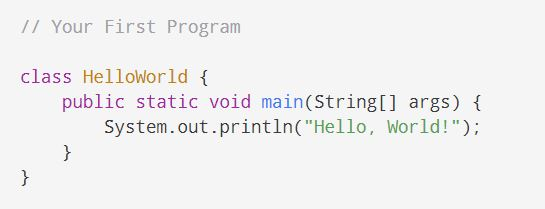
\includegraphics[width=1\linewidth]{images/helloWorldJava.JPG}
        \caption{Java Implementation of "Hello, World!" Program
    }
    \label{fig:helloWorldJava} 
\end{figure}

When put into the j2py Translator, the Python source code in figure \ref{fig:helloWorldJ2py} was given.

\begin{figure}[htb]
    \centering
    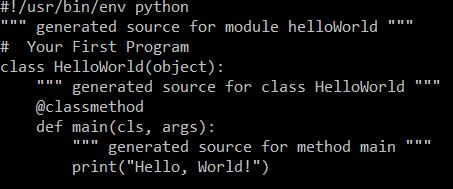
\includegraphics[width=1\linewidth]{images/helloWorldJ2py.JPG}
        \caption{J2py python source code output from figure \ref{fig:helloWorldJava} input
    }
    \label{fig:helloWorldJ2py} 
\end{figure}

Whilst this output is accurate and will produce the desired output when ran on a python compiler, it is also ridiculously long winded. The simplest "Hello, World!" program in Python would require just one line: print("Hello, World!"). This is because python does not require the class and method declaration that Java does, since it does not enforce OOP.
It is good practice however to enforce Object-Oriented Programming, as it makes code reusable and makes coding easier when working with larger programs. Even when OOP principles are enforced however, the translation can be as simple as shown in figure \ref{fig:helloWorldPy}:

\begin{figure}[htb]
    \centering
    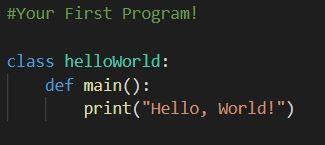
\includegraphics[width=1\linewidth]{images/helloWorldPy.JPG}
        \caption{Simplest OOP form of the "Hello, World!" Python Program
    }
    \label{fig:helloWorldPy} 
\end{figure}

This is the simplest example of how it was decided that J2Py's translations were overly confusing and wordy, and turned the simplest example of code into several lines, many of which were futile. One common programming principle is "Keep It Simple Stupid" or KISS, which states code should be as clean, efficient, understandable and maintainable. This principle did not seem to be applied to the j2py translations, and if this example of simple code turned 3 lines of code into 9 lines, you can assume that with longer code scripts, the amount of excess code will grow further, making the translations more difficult to comprehend.

Another issue with J2Py is the fact that it was built for Python version 2.7, as stated on their gitHub repository documentation. The Java2Python download instructions on their gitHub give directions on how to install Java2Python version 0.5.1, which is the version that was initially used for testing. Within their configuration file (used to give the python translation), the print command did not have parentheses around the statement being printed. This meant technically that any translated code that had print commands in them, could not be compiled in python3. Given that we are now on python version 3.9, this makes the configuration file outdated. Whilst it was a relatively simple change to make, someone who is not used to working in programming may have struggled to make the changes that were required in the configuration file, meaning they would have to manually go back and add parentheses to their print statements which would be time consuming, especially in longer translated code.

Another criticism I had of Java2Python was it's lack of extendibility. Java2Python does a great job of offering translations of a bunch of simple/standard coding paradigms, however if using j2py for a certain task, the option of adding a translation, or even altering a translation to fit with the intended output, is desirable. J2Py does offer customization in the form of a command line alteration, however it is difficult to understand how to use that effectively, or how to add a new coding paradigm altogether. A more desirable feature would have been a template engine which is easier for user to understand, alter, and extend.

One final thing I would mention about J2Py is its efforts to translate imports. Although this is very difficult since Java and python will not share a lot of mutual libraries, J2Py makes no effort to translate Java packages to Python. This would be a cool feature if possible, which over time if added to effectively, could make the tool far more powerful.

\section{Requirements}
Given what was found from the background reading and the deep dive into the Java2Python the requirements of the project were shaped accordingly. There was now a general consensus on how the tool should be built, with certain design ideas in mind as well as a realistic end goal in mind.

\subsection{Minimum Viable Product}
The minimum viable product (MVP) is the absolute minimum requirement for the project to be able to achieve before it can be considered a success. For this I would refer back to a couple of the objectives mentioned in section 1.4 of the Introduction. Firstly the translator should be able to translate simple/common coding paradigms, which were defined as follows:
\begin{itemize}
    \item
    Conditional statements in the form of if/else/ else if as well as logical conditions using mathematical symbols (e.g 'a>'b, 'a<b', 'a==b').
    \item
    Switch statements, which are a form of conditional statement to select a block of code that executes if a case is met (switch/case/default)
    \item
    While loops, and do/while loops where a block of code will be executed as long as a specified condition is reached.
    \item
    For loops, where the number of times code will be looped is specified, rather than a condition waiting to be met. Also for-each loops can be used when looping through elements in a list-type structure such as an array.
\end{itemize}

Since this would technically be nothing new, since j2py already has these capabilities, the second objective should also be considered for the MVP: to ensure the code is expandable for future work. This would mean even if the MVP did not surpass the capabilities of other translators, it had the capabilities to be added to with an intuitive design. Additionally, with reference to the forth objective, the translation should be as simplified as possible. This means that if it was to only be the simplest paradigms as listed above, they would all be translated into the simplest form.

\subsection{Next Level of Requirements}
This section describes what should be prioritised once the MVP has been implemented.

\subsubsection{Translation Capabilities} In an ideal world, this tool would be able to translated every Java source code script to Python source code with 100\% accuracy. Given what is known about language translation however, the next step after MVP would be to have the whole unimplemented Java grammar translatable to Python. By this, we mean the full syntax of Java would be translatable outwith syntax that can be added from imported libraries. For a brief overview, this would involve classes, methods, interfaces, try/catch statements, clauses, enumeration and annotations.

\subsubsection{Accessibility}
The language translator has to be simple enough to use, since it's primary function is making code migration easier. One feature of j2py which was admirable was it's simple command line input. This was something held in relatively high priority for this translator, as it was decided a user interface was not particularly required, but that shouldn't mean a list of confusing commands were required, otherwise it could become more effort than the translation is worth. Instead the command line input should be simple and intuitive.

\subsubsection{Explanation of Failure}
Due to the inevitability of translations occasionally failing, this tool should be able to offer an explanation as to where translation has failed. This could be done as simply as replacing the translated line with internal commentary. This means that the user knows what has to be translated manually and where.

\subsubsection{Enforcing OOP}
As mentioned previously when critiquing the J2py tool, Python code does not always have to be in OOP form, but it is often good coding practice to do so. Ideally, the code should keep a similar structure to the java file in terms of classes and methods to make it easier to understand how stuff has been translated. There are also advantages to OOP programming such as reusability, which helps programmers stick to the Don't Repeat Yourself (DRY) principle.

\subsection{Desirable Features}
This section describes features of the translator which may be slightly outwith the scope of this project but would be ideal features to be available in this tool.
\subsubsection{Dealing with Imports}
The possibility of doing this with any form of accuracy is low since Python and Java's imported packages are so different, however if possible it would be very effective if the packages the Java script imports could be mapped to the same or a similar package in Python with the same features. Focus would be on mathematical and statistical packages as they are the most commonly utilised packages in either language. (https://www.programcreek.com/2011/08/the-most-widely-used-java-apis/)

\subsubsection{Coding Style Transformation}
This is a feature which may not be too difficult to implement however is far from a requirement. There are a lot of stylistic differences between how people prefer to code in Java and Python. One example of this is Java users tend to prefer camelCase naming style (according to Oracle), while Python prefer to use underscoring (According to PEP8 - Python Code Style Guide). For example, a variable titled 'firstName' in java would usually be titled 'first\_name' if titled by a Python developer. Using the standard style of a programming language can often be useful but generally is not that import and so is a low priority feature.

\subsubsection{Reverse Translation}
One feature which may be very helpful is reverse translation so that the tool can also translate from Python to Java. With the research done into translation however it would appear this is twice as much work. This is because that would involve defining two different grammars which can be very time consuming and then defining the targeted output in Java. There are also issues when translating from Python to Java such as variable typing, and visibility modifiers.

\subsubsection{Other Languages}
The possibility to translate from Java to another target language is also a desirable feature of this translation tool. Given the time and resource constraint, it was easiest to focus on ensuring the translation from Java to Python was effective and accurate. However the insertion of another target language would make this tool very powerful, but is slightly beyond the realm of possibility.




\todo{What is the problem that you want to solve, and how did you arrive at it?}
\section{Guidance}
Make it clear how you derived the constrained form of your problem via a clear and logical process. 

The analysis chapter explains the process by which you arrive at a concrete design. In software 
engineering projects, this will include a statement of the requirement capture process and the
derived requirements.

In research projects, it will involve developing a design drawing on
the work established in the background, and stating how the space of possible projects was
sensibly narrowed down to what you have done.

%==================================================================================================================================
\chapter{Design}
This project used iterative design processes when developing the translation tool. This meant implementing small sections of the tool, testing, and then going back to the design phase should limitations occur. It was imperative that the limitations of the technology choices were known early in implementation as it was time consuming to build a full system and so testing the capabilities early on was vital. This chapter will describe the agreed upon final design of the translator which was chosen after some trial and error with implementation, however due to the fail-fast nature of this project, the tool was designed in one main iteration. There will be a section for each design decision that was made in regard to the translation tool. This will be structured from the start of the user's translation process to the end of the translator process. Any design decisions that are unclear will most likely be justified when the technologies are described in more detail in chapter 5, the implementation phase.

\section{Translation Entry Point}
As mentioned in the requirements chapter, to use a translator, an interface is not necessary; a command line instruction is sufficient. The design of the command line instruction should be as simple yet informative as possible. The surrounding code was arbitrary dependent on the chosen technology for implementation, but some input material was crucial. 

Firstly, the input should include the title of the java source code being translated. The fact the instruction takes place on a command line means this syntax can be used to navigate to the desired file, using slashes and ellipses to navigate between directories. 

Secondly, the input should include the desired output language. Although the primary intention of this project was to translate to Python, in the interest of making the translator expandable, this is a good feature. If in future, the translator was to be able to translate to another programming language, you could insert a different target language here instead of Python. This input is not required however, and if left blank, the translator will assume Python is the target.

Third and finally, the input should include the destination for the translated code. If given, the output of the translation will be written to the given file. This file does not need to exist prior to the translation process. If a destination file is not given, the translation will just be output in the terminal window. If the destination file is given with a python extention i.e "output.py" then it will be executable, otherwise it will just be a standard text file.

This means that the only \textbf{required} input is the input source code, and that any of the following inputs would be permitted:

\textbf{input.java python output.py}

\textbf{input.java python}

\textbf{input.java output.py}

\textbf{input.java}

\section{Input Processing}

The design for processing the input involved two processes called lexical analysis and parsing. The translator has a Java grammar file which maps out the parser and lexer rules to give meaning to the java source code being processed. The general idea is that the lexer will scan the input and tokenize it, breaking the input into smaller objects and giving these objects meaning. The parser will then scan through these 'tokens' and produce the 'parsing result'. A good example of how a parser and lexer work is given below, sourced at 'A Guide to Parsing: Algorithms and Terminology'.

\begin{figure}[htb]
    \centering
    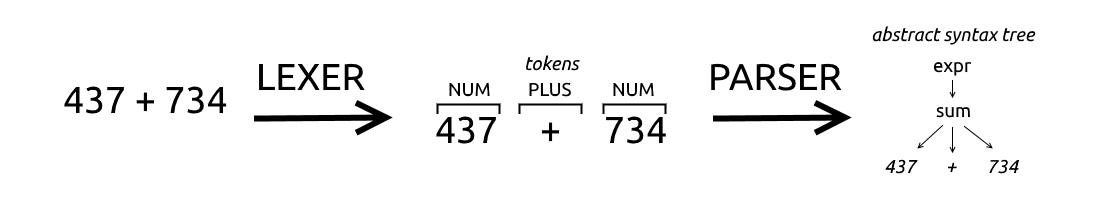
\includegraphics[width=1\linewidth]{images/parserLexer.png}
        \caption{Example of how lexical analysis and parsing work. From 'A Guide to Parsing: Algorithms and Terminology'
    }
    \label{fig:parserLexer} 
\end{figure}

From this example, the lexer is able to recognise that '437' and '734' are tokens of type NUM and '+' is a token of type PLUS. This would be defined in the grammar file as a lexer rule.
The parser is then able to recognise that if those three tokens appear in that order then a sum expression is being displayed. This would be defined as a parser rule in the grammar file.
Parsers often produce abstract syntax trees, as shown in figure \ref{fig:parserLexer} to represent the syntactical structure of the source code.

To give a more programming language based example, we could take an if-statement. Say the following pseudocode appeared:

\textbf{if (a>b)
    print(a)}

An AST is shown in figure \ref{fig:ifStatAST} (this was all generated by hand and so does not reflect the exact lexing or parsing process that was implemented in our product). As the diagram shows, each element of the statement was tokenised in the lexer process. The parser was then able to recognise patters of tokens appearing together, and generated parsed results. Certain elements may be parsed further, for example, once the tokens for "a>b" were parsed, the result became a "COMPARISON" token which was then able to be parsed further in the if-statement. 
This is roughly how the Java source code is first processed by the translator.

\begin{figure}[htb]
    \centering
    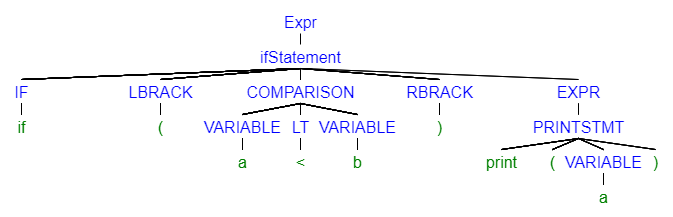
\includegraphics[width=1\linewidth]{images/ifStatAST.png}
        \caption{AST generated for the if-statement pseudocode
    }
    \label{fig:ifStatAST} 
\end{figure}.

\section{Processing the Translation}
To output the Python source code, the results from the parser are used, along side a template engine.  The template engine technology was a choice made due to the extendibility objective, as the technology made it far easier to customize and add to the output, which was a criticism of the J2Py translator. More information of how and why this was easier will be given in the implementation chapter. As mentioned in the analysis and Requirements chapter, an intermediate layer seemed necessary for a programming language translator tool. The intermediate layer essentially exists as the result of the input processing (tokenized output and parsing results). From this stage the processed information works directly with the template engine, since the template rules follow the same naming conventions as the parser rules, and the parameters of the template rules are the tokens. This can be easily seen via syntax as shown in figures \ref{fig:grammarSyntax} and \ref{fig:templateSyntax}, however further explanation of syntax will be explained when technologies are discussed in the implementation chapter.

\begin{figure}[htb]
    \centering
    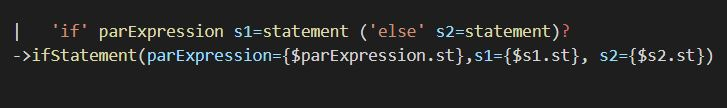
\includegraphics[width=1\linewidth]{images/grammarSyntax.JPG}
        \caption{Grammar Syntax for an If-statement
    }
    \label{fig:grammarSyntax} 
\end{figure}.

\begin{figure}[htb]
    \centering
    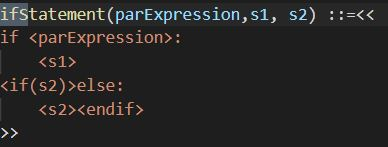
\includegraphics[width=1\linewidth]{images/templateSyntax.JPG}
        \caption{Template Engine Syntax for an if-statement
    }
    \label{fig:templateSyntax} 
\end{figure}.

As shown from figure \ref{fig:grammarSyntax}, An if statement takes in a parExpression token, and a statement token, and then has the option of a second statement token, if there is an else clause in the if-statement. The grammar then calls the template engine through the arrow, where a ifStatement rule is called, and passes the tokens in as parameters.
Figure \ref{fig:templateSyntax} then shows the declaration of the ifStatement rule, taking the tokens in as parameters. The template is how such a rule should be presented in Python, and places the parameters accordingly. The <if(s2)> syntax that can be seen checks if there is an else-clause, and if so adds some python source code, if not this code will not be output.

Translation is considered complete when every parsed result has been through it's respective template rule in the engine, and the result is ready to be output.


\section{Presenting Output}
As briefly mentioned in section 4.1, once the translation has been complete, it will display in the terminal window. It will also be written to a file if specified in the initial command request. One consideration for the tool to take it one step further was to compile the output to see if the python code can run. The tool does not do this however for a number of reasons. Firstly, the technology choices made this particularly difficult, but this will be discussed in the implementation chapter. On top of this, the primary aim for this tool was to produce some form of syntactical translation from Java to Python, and so syntax was prioritised over correctness. This means the tool is by no means guaranteeing working python source code, but is instead guaranteeing something to work with in the form of a syntactical translation. 





\todo{How is this problem to be approached, without reference to specific implementation details?} 
\section{Guidance}
Design should cover the abstract design in such a way that someone else might be able to do what you did, 
but with a different language or library or tool. This might include overall system architecture diagrams,
user interface designs (wireframes/personas/etc.), protocol specifications, algorithms, data set design choices,
among others. Specific languages, technical choices, libraries and such like should not usually appear in the design. These are implementation details.


%==================================================================================================================================
\chapter{Implementation}
This chapter will cover the implementation phase of the project. This will largely reference how the design mentioned in the previous chapter was implemented. There will also be detail into how readily available open-source code was utilised and manipulated to fit the project, and detailed justification on any technology decisions that were made.

\section{Processing Input - ANTLR}
Early on in this project it had became clear that building a translation tool from scratch would me a monumental task. For this reason it was important to take as deep a dive as possible into the existing technologies and frameworks that would ease this project. ANTLR was a framework that was often coming up; not only was it used in the java2python translator we analysed and critiqued in detail, it was also referenced in several papers, and had been used in coursework for the University of Glasgow Programming Languages (H) course. 
ANTLR is a parser generator tool, which can be used to read, process, execute or translate structured text. It is widely used in academia and industry to make languages, tools and frameworks including twitter search using it for query parsing.

ANTLR takes a formal language description called a grammar, and generates a parser for that language that can automatically build parse trees. Parse trees are data structures showing how a grammar matches the input. 
As stated in the design process, A parser is how we intended to process the input Java source code. ANTLR was a tool that would be able to do this automatically and prevent a manual parser from being built, which would take a lot of time and effort.

As mentioned in ANTLR's documentation, it is a widely used software tool and thus, has a large community of users online. This meant resources for using ANTLR are very readily available. The ANTLR gitHub account has several repositories which allows users to contribute. Some of these include repositories called "grammars-v3" and "grammars-v4" which includes the formal language description of popular programming languages, including Java. These were grammar files of the core/unimplemented versions of Java, which were over 2000 lines long. These grammars are licensed and copyrighted by Terence Parr, creator of ANTLR, and so are trustworthy resources.

"Java.g" from the "grammars-v3" repository was used in this project. It had to be altered and extended for use in this project however having this initial grammar there saved a lot of time and inaccuracies that may have occurred if the grammar file was to be created manually. The reasoning for using an older grammar file will be discussed later in this chapter when we discuss the translation of the parse trees.

\section{Translation Technology}

\subsection{ANTLR Listener}
Once it was decided upon that ANTLR was to be used for the initial parsing of the Java source code, it was important to figure out how these parsed results would be converted into Python source code. Defined as a tool to be used for translation, it was assumed that these capabilities already existed in ANTLR. To try and find out more about ANTLR's translator capabilities, "The Definitive Antlr 4 Reference" was examined. This is a large, informative book which guides ANTLR users on how to solve language recognition problems. The guide has a chapter titled "Building a Translator with a Listener" which obviously peaked our interest, as we intended on building a translator. The instructions were clear and very informative, however seemed to be producing some pretty verbose code, for the amount of code being translated. On top of this, we wanted the design of the translator to be as intuitive as possible, so that it can be worked on in the future with as little confusion as possible.

\subsection{StringTemplate}
Due to the concerns expressed in the previous section, it was decided that different approaches to translation via ANTLR should be explored. This is when an article originally written by Terence Parr, creator of ANTLR, was discovered. This paper was titled "Language Translation Using ANTLR and StringTemplate". StringTemplate is a java template engine which is able to generate source code, along with other formatted text output. StringTemplate was actually used to generate ANTLRv3. This paper described how ANTLR was used to create the grammar for a simplified version of C, called Cminus or "C-". It then used stringTemplate technology to "unparse" the parsed Cminus input, into 3 different target languages; Java, Python and the "radically different" psuedo bytecodes.

Instantly it became clear that approach made a lot more sense since the syntax was far more intuitive, and so the decision was made to use stringTemplate technology. The next subsection will give a comparison of the two to further justify this decision.

\subsection{ANTLR Listener vs StringTemplate}
In order to prove that the StringTemplate approach made more sense than the ANTLR Listener, I shall demonstrate the translation the Listener was carrying out in "The Definitive ANTLR 4 reference" and then show how it would be done using StringTemplate.

The example being being given in this book is translating a Java Class into a Java Interface. The areas of the Java grammar which this translation concerns are given in the book and are shown in figure \ref{fig:javaGrammarExample}

\begin{figure}[htb]
    \centering
    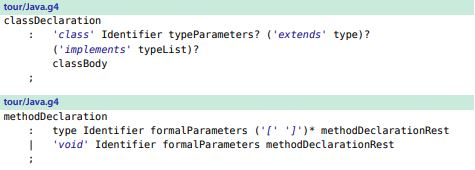
\includegraphics[width=1\linewidth]{images/javaGrammarExample.JPG}
        \caption{java grammar extract showing the definition of a class declaration and a method declaration
    }
    \label{fig:javaGrammarExample} 
\end{figure}.

This is the basic grammar which will be used by both the stringTemplate translation and the ANTLR listener translation, since this is just the input parsing process. The grammar does have to be edited slightly for the stringTemplate, to essentially call the template rules. This can be seen in figure \ref{fig:STAlteration}

\begin{figure}[htb]
    \centering
    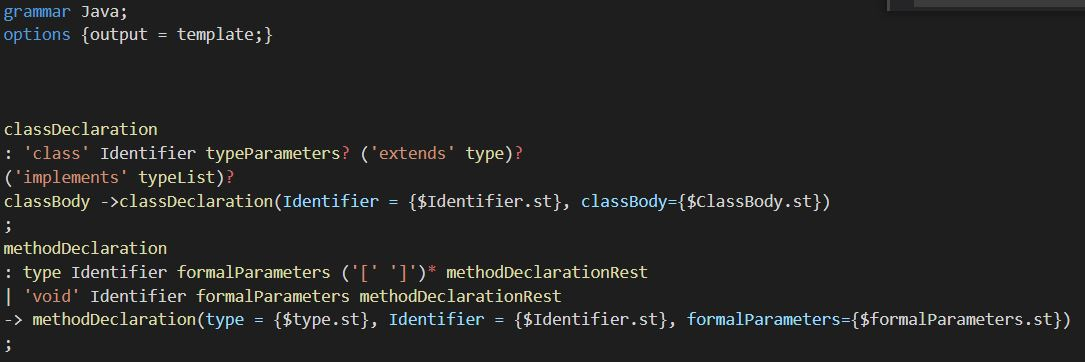
\includegraphics[width=1\linewidth]{images/STAlteration.JPG}
        \caption{The Alterations made to the grammar in order for stringTemplate to operate
    }
    \label{fig:STAlteration} 
\end{figure}.

As you can see there is slightly more syntax here, but it is all very self explanatory, and all it does is pass the appropriate tokens to the template rule to be unparsed. Additionally, the "output = template" line has to be added, in order for the program to understand why this extra syntax is there, when auto generating parsers.

Both versions of the translator require a main program, which will launch the application. I will not give an example here as the syntaxes are very similar up until the parser has been launched. The only difference comes when the listener is called and walked or when the template is applied and displayed, however both these processes are only a couple of lines long, and so there is no big difference to compare.

The main difference comes however when it comes to actually launching the translation. Figure \ref{fig:STExtractor} shows how the stringTemplate implementation for the translation would look, whilst Figure \ref{fig:ListenerExtractor} shows the syntax for the ANTLR Listener implementation.

\begin{figure}[htb]
    \centering
    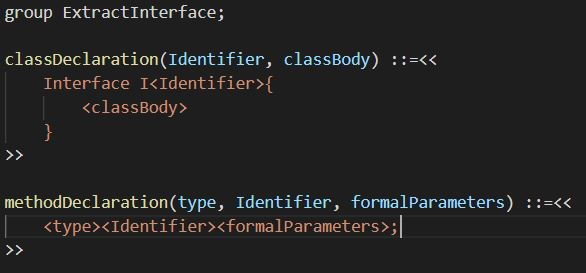
\includegraphics[width=1\linewidth]{images/STExtractor.JPG}
        \caption{The StringTemplate for translating a Java Class into a Java Interface
    }
    \label{fig:STExtractor} 
\end{figure}.

\begin{figure}[htb]
    \centering
    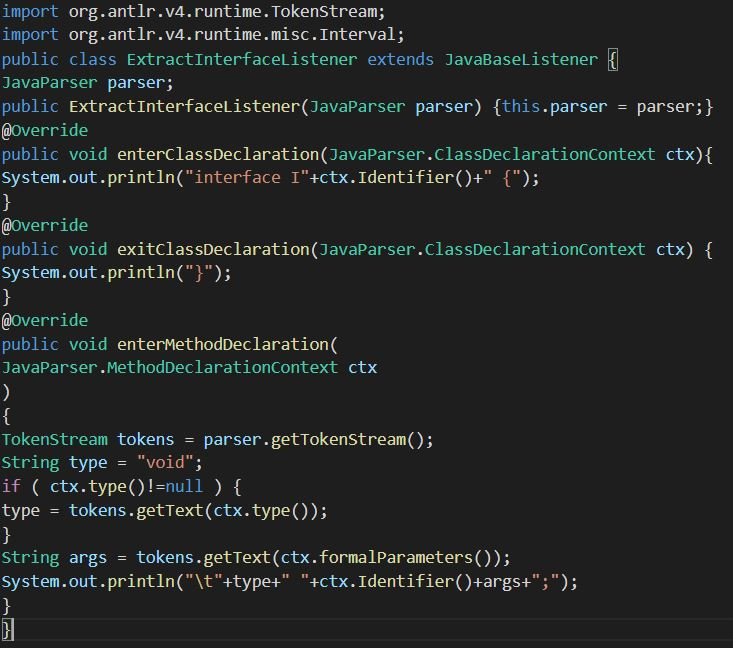
\includegraphics[width=1\linewidth]{images/ListenerExtractor.JPG}
        \caption{The ANTLR Listener script for translating a Java Class into a Java Interface
    }
    \label{fig:ListenerExtractor} 
\end{figure}.

To clarify how each process works, the stringTemplate main program will insert the relevant template before the parser runs. This means that as the source code is parsed using the grammar file, when a parsed result is found (i.e a classDeclaration or methodDeclaration), the template operation is called, from the additional syntax we added to the grammar in figure \ref{fig:STAlteration}. From there, as figure \ref{fig:STExtractor} shows, the syntax is very self explanatory and the templates are essentially copied and the tokens from the grammar are directly plugged into the templates. This syntax I feel is very self explanatory and intuitive, as it is clear where alterations would be made if required. For the sake of transparency, the classBody parameter could be anything that appears within the class, however in the instance of this example, it is 3 method declarations. The identifier is the name of the class or method being declared, the type is the type of object being returned by the method, and the formalParameters are the parameters being passed into the method being declared.

The ANTLR listener does the parsing and translating seperately compared to the stringTemplate example. Firstly the main program parses the source code using the auto generated parser from the grammar, and a parse tree is built. Next a walker and an instance of the extractInterfaceListener are declared within the main program. This allows the nodes of the parse tree that has been built to be visited, and if a node matches one of the methods that have been overridden in the listener, then this method will be called, outputting the altered syntax.

Both methods are really innovative ways of translation and there is definitely an argument for either to be used. The ANTLR listener technique is effective for seperation of concerns between the parsing of the source code and the parse application. With reference to the intended outcomes for this project however, it was very important that this tool was extendible and adaptable, and the intuitve interface of the stringTemplate approach allowed that. The verbosity of the listener Java script was off-putting and it was often difficult to access the intended object (for example, to access the identifier token from the Class Declaration, the object type would be "JavaParser.ClassDeclarationContext.Identifier()", and the objects only got more confusing the more buried they were in the Java grammar. One glance at figure \ref{fig:STExtractor} however and the syntax is relatively easy to understand and not overly bulky. Also, the convenience of the stringTemplate rules being directly called from the Java grammar outweighed the advantages that come with seperating concerns.

With this pros and cons comparisons weighed out, it was decided that combining ANTLR with StringTemplate was the technological approach that would be used.

\subsection{Outdated Technology}
When building a new software tool, it is natural to decide to use the most up to date technologies to do so. For this reason, we instantly began looking at StringTemplatev4 and ANTLR4, the most up to date versions of each technology.

To try and work out the key differences, gitHub was searched for examples of ANTLR4 and StringTemplatev4 interacting to use for reference. The search was unsuccessful and it seemed as if gitHub did not have any repositories consisting of these two technologies working together. The Definitive ANTLR 4 Reference guide which had been used for the ANTLR Listener example was then used to try and find some StringTemplate usage. Unfortunately, it seemed as if ANTLR had moved away from using stringTemplate as a translation target, and thus would be difficult to use for this project.

ANTLR4 was build again from scratch after ANTLRv3 and so it was clear that the technology had undergone a massive change. StringTemplate's wiki on gitHub states that it was used to develop ANTLRv3 and so, it was clear perhaps these technologies had a lot more in common. Fortunately, ANTLRv3 still has an active repository, and the source code from the paper which was referenced earlier titled "Language Translation Using ANTLR and StringTemplate", was given in the examples folder. After examining the source code it was decided that this was the cleanest way to implement a translator and it fit the objectives for this project to be intuitive and expandible if it was to be worked on in the future. 

With that in mind, we felt that using older technologies to build our tool was a justified decision. Furthermore, the older ANTLR and StringTemplate versions does not prevent us from implementing the newest versions of Python or Java, and so this tool will still be relevant, despite being build using older backend software.

\section{Translation Implementation}
As mentioned in section 5.1, the ANTLR resources were vast and so the majority of the grammar implementation was already done. The additional alterations seen in figure \ref{fig:STAlteration} were required, which took a long time to implement due to the size of the grammar file. This task was more tedious than difficult however.

For each parsed object, I pass every token from the object to the stringTemplate operation, even if it isn't required for the python version of the object. For example, when declaring a variable in java, it could require a modifier, a type, an identifier name, and a declaration (whether that means declaring the variable and setting it's value later or setting it's initial value as it's declared). In Python however, variables are dynamically typed. This means that the modifiers and types are not essential to be passed into the StringTemplate to be unparsed. We do this however, due to extendibility aim of our project. If in the future we were to extend the translator to include a C# template for example, we will need the modifiers and types, and thus we won't need to modify the grammar file again if the tokens are still being passed into the template operation.

In contrast to the Java grammar file, the Python stringTemplate file had to be built near enough from scratch. It was important to us to prioritise making the translation as syntactically accurate and as clean and simple as possible. For this reason I used Python resources online instead of my own interpretation of Python, primarily the extended Python tutorial on w3Schools.com. There was however a few edge cases where the Java and Python implementations would vary quite a lot and the translation would have to be very much improvised.

\subsection{The Java Switch Statement}
One very popular expression in Java is the Switch statement. The switch statement is used to select one of many code blocks to be executed. The switch expression is evaluated once and the expressions value is compared to the value of each case. If the values match, the associated block of code is executed. The break and default keywords are often also used within switch statements. The 'break' keyword is often used at the end of a case's associated code to break out of the switch block. The 'default' keyword is used in the case where there is no case match, and gives some code to run instead. An example of this java source code is given in figure \ref{fig:switchJava}.

\begin{figure}[htb]
    \centering
    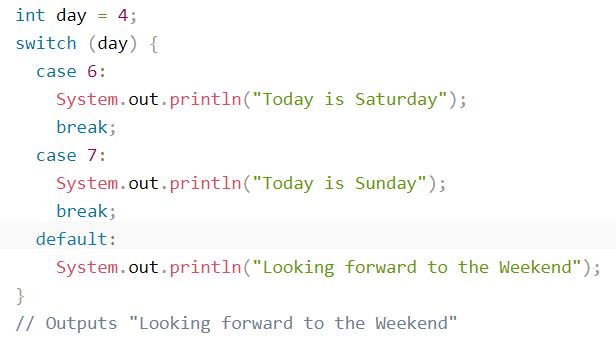
\includegraphics[width=1\linewidth]{images/switchJava.JPG}
        \caption{A switch expression in Java
    }
    \label{fig:switchJava} 
\end{figure}.

Python does not offer the option of a switch expression, however this is a common coding pattern in Java and so wanted the translator to be able to interpret this in some way. To get around this issue, we made use of if/else/elif in Python. This was inspired by the j2py translator which also translated a switch expression in this way. This meant that the java source code in figure \ref{fig:switchJava} was translated to the Python source code shown in figure \ref{fig:switchPython}

\begin{figure}[htb]
    \centering
    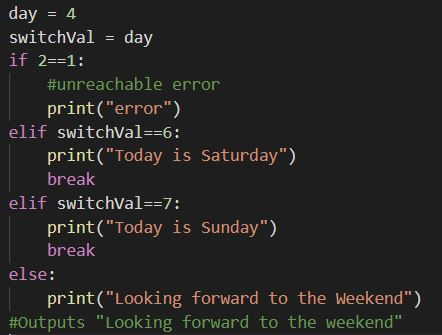
\includegraphics[width=1\linewidth]{images/switchTranslation.JPG}
        \caption{The resulting translation from the switch expression
    }
    \label{fig:switchPython} 
\end{figure}.

The majority of this translation is quite self explanatory; the elif statements replaced the case statements, and the else statement replaced the default statement. There are one or two parts of this translation that still need explained however, which will address one of the minor issues with the stringTemplate method of implementation.
The way the Java grammar defines a lot of code patterns is into several different parts. For this example, the switch statement is broken into switchStatement, switchBlockStatementGroups, switchBlockStatementGroup, and switchLabel. The switchStatement encapsulates the whole switch block of code. The switchBlockStatementGroups is all of the switchBlockStatementGroup objects grouped together. The switchBlockStatement group encapsulates each block from the switchLabel to the end of that chunk of code, usually the break keyword. The switchLabel is either the case or the default keyword in Java, meaning it is either elif or else in the Python translation. 
Because of this fragmentation, certain parameters are not accessible from the template method. For example, switchVal has to be definied, because the switchBlockStatement group has no access to the name of the variable that is being compared. There also has to be an empty if statement at the start of the block, as it is impossible to tell using stringTemplate which is the first switchBlockStatementGroup, and so all of them have to have their switchLabel set to the elif keyword.

\subsection{the for loop (example of making syntax easier)}

\section{Output}
\section{Walkthrough of example (from source code, through grammar, showing string template, showing output)}




\todo{What did you do to implement this idea, and what technical achievements did you make?}
\section{Guidance}
You can't talk about everything. Cover the high level first, then cover important, relevant or impressive details.

\section{General guidance for technical writing}

These points apply to the whole dissertation, not just this chapter.

\subsection{Figures}
\emph{Always} refer to figures included, like Figure \ref{fig:relu}, in the body of the text. Include full, explanatory captions and make sure the figures look good on the page.
You may include multiple figures in one float, as in Figure \ref{fig:synthetic}, using \texttt{subcaption}, which is enabled in the template.


% Figures are important. Use them well.
\begin{figure}[htb]
    \centering
    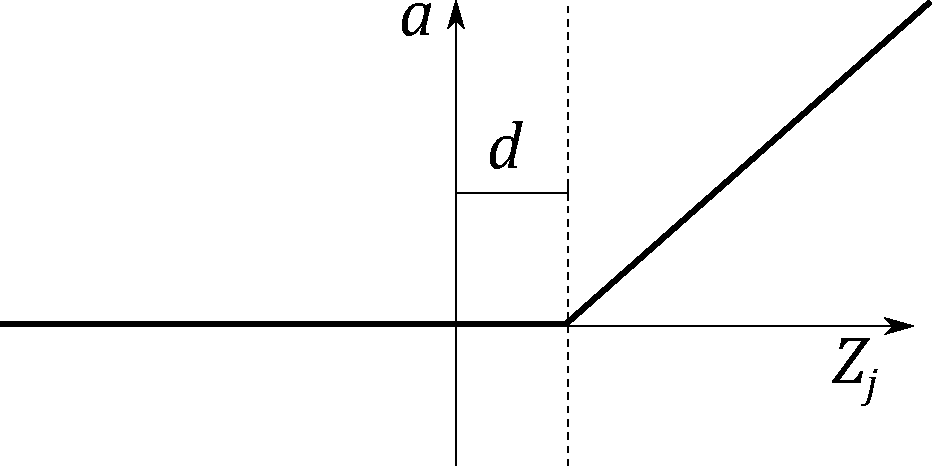
\includegraphics[width=0.5\linewidth]{images/relu.pdf}    

    \caption{In figure captions, explain what the reader is looking at: ``A schematic of the rectifying linear unit, where $a$ is the output amplitude,
    $d$ is a configurable dead-zone, and $Z_j$ is the input signal'', as well as why the reader is looking at this: 
    ``It is notable that there is no activation \emph{at all} below 0, which explains our initial results.'' 
    \textbf{Use vector image formats (.pdf) where possible}. Size figures appropriately, and do not make them over-large or too small to read.
    }

    % use the notation fig:name to cross reference a figure
    \label{fig:relu} 
\end{figure}


\begin{figure}[htb] 
    \centering
    \begin{subfigure}[b]{0.45\textwidth}
        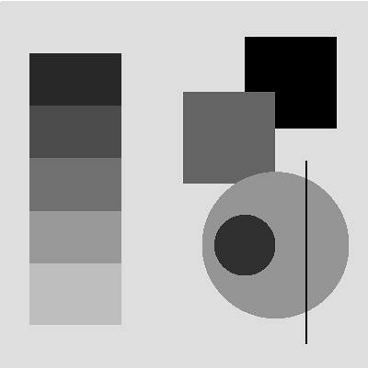
\includegraphics[width=\textwidth]{images/synthetic.png}
        \caption{Synthetic image, black on white.}
        \label{fig:syn1}
    \end{subfigure}
    ~ %add desired spacing between images, e. g. ~, \quad, \qquad, \hfill etc. 
      %(or a blank line to force the subfigure onto a new line)
    \begin{subfigure}[b]{0.45\textwidth}
        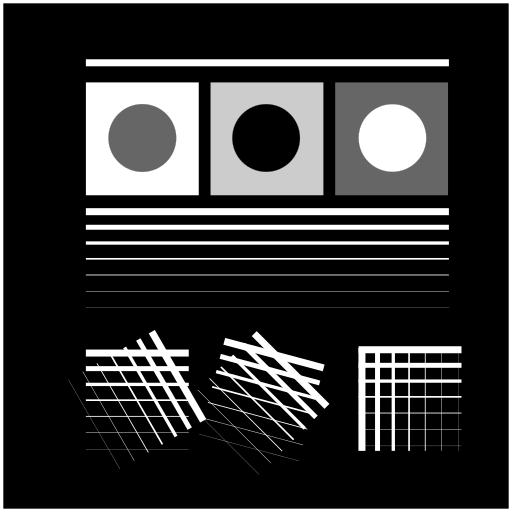
\includegraphics[width=\textwidth]{images/synthetic_2.png}
        \caption{Synthetic image, white on black.}
        \label{fig:syn2}
    \end{subfigure}
    ~ %add desired spacing between images, e. g. ~, \quad, \qquad, \hfill etc. 
    %(or a blank line to force the subfigure onto a new line)    
    \caption{Synthetic test images for edge detection algorithms. \subref{fig:syn1} shows various gray levels that require an adaptive algorithm. \subref{fig:syn2}
    shows more challenging edge detection tests that have crossing lines. Fusing these into full segments typically requires algorithms like the Hough transform.
    This is an example of using subfigures, with \texttt{subref}s in the caption.
    }\label{fig:synthetic}
\end{figure}

\clearpage

\subsection{Equations}

Equations should be typeset correctly and precisely. Make sure you get parenthesis sizing correct, and punctuate equations correctly 
(the comma is important and goes \textit{inside} the equation block). Explain any symbols used clearly if not defined earlier. 

For example, we might define:
\begin{equation}
    \hat{f}(\xi) = \frac{1}{2}\left[ \int_{-\infty}^{\infty} f(x) e^{2\pi i x \xi} \right],
\end{equation}    
where $\hat{f}(\xi)$ is the Fourier transform of the time domain signal $f(x)$.

\subsection{Algorithms}
Algorithms can be set using \texttt{algorithm2e}, as in Algorithm \ref{alg:metropolis}.

% NOTE: line ends are denoted by \; in algorithm2e
\begin{algorithm}
    \DontPrintSemicolon
    \KwData{$f_X(x)$, a probability density function returing the density at $x$.\; $\sigma$ a standard deviation specifying the spread of the proposal distribution.\;
    $x_0$, an initial starting condition.}
    \KwResult{$s=[x_1, x_2, \dots, x_n]$, $n$ samples approximately drawn from a distribution with PDF $f_X(x)$.}
    \Begin{
        $s \longleftarrow []$\;
        $p \longleftarrow f_X(x)$\;
        $i \longleftarrow 0$\;
        \While{$i < n$}
        {
            $x^\prime \longleftarrow \mathcal{N}(x, \sigma^2)$\;
            $p^\prime \longleftarrow f_X(x^\prime)$\;
            $a \longleftarrow \frac{p^\prime}{p}$\;
            $r \longleftarrow U(0,1)$\;
            \If{$r<a$}
            {
                $x \longleftarrow x^\prime$\;
                $p \longleftarrow f_X(x)$\;
                $i \longleftarrow i+1$\;
                append $x$ to $s$\;
            }
        }
    }
    
\caption{The Metropolis-Hastings MCMC algorithm for drawing samples from arbitrary probability distributions, 
specialised for normal proposal distributions $q(x^\prime|x) = \mathcal{N}(x, \sigma^2)$. The symmetry of the normal distribution means the acceptance rule takes the simplified form.}\label{alg:metropolis}
\end{algorithm}

\subsection{Tables}

If you need to include tables, like Table \ref{tab:operators}, use a tool like https://www.tablesgenerator.com/ to generate the table as it is
extremely tedious otherwise. 

\begin{table}[]
    \caption{The standard table of operators in Python, along with their functional equivalents from the \texttt{operator} package. Note that table
    captions go above the table, not below. Do not add additional rules/lines to tables. }\label{tab:operators}
    %\tt 
    \rowcolors{2}{}{gray!3}
    \begin{tabular}{@{}lll@{}}
    %\toprule
    \textbf{Operation}    & \textbf{Syntax}                & \textbf{Function}                            \\ %\midrule % optional rule for header
    Addition              & \texttt{a + b}                          & \texttt{add(a, b)}                                    \\
    Concatenation         & \texttt{seq1 + seq2}                    & \texttt{concat(seq1, seq2)}                           \\
    Containment Test      & \texttt{obj in seq}                     & \texttt{contains(seq, obj)}                           \\
    Division              & \texttt{a / b}                          & \texttt{div(a, b) }  \\
    Division              & \texttt{a / b}                          & \texttt{truediv(a, b) } \\
    Division              & \texttt{a // b}                         & \texttt{floordiv(a, b)}                               \\
    Bitwise And           & \texttt{a \& b}                         & \texttt{and\_(a, b)}                                  \\
    Bitwise Exclusive Or  & \texttt{a \textasciicircum b}           & \texttt{xor(a, b)}                                    \\
    Bitwise Inversion     & \texttt{$\sim$a}                        & \texttt{invert(a)}                                    \\
    Bitwise Or            & \texttt{a | b}                          & \texttt{or\_(a, b)}                                   \\
    Exponentiation        & \texttt{a ** b}                         & \texttt{pow(a, b)}                                    \\
    Identity              & \texttt{a is b}                         & \texttt{is\_(a, b)}                                   \\
    Identity              & \texttt{a is not b}                     & \texttt{is\_not(a, b)}                                \\
    Indexed Assignment    & \texttt{obj{[}k{]} = v}                 & \texttt{setitem(obj, k, v)}                           \\
    Indexed Deletion      & \texttt{del obj{[}k{]}}                 & \texttt{delitem(obj, k)}                              \\
    Indexing              & \texttt{obj{[}k{]}}                     & \texttt{getitem(obj, k)}                              \\
    Left Shift            & \texttt{a \textless{}\textless b}       & \texttt{lshift(a, b)}                                 \\
    Modulo                & \texttt{a \% b}                         & \texttt{mod(a, b)}                                    \\
    Multiplication        & \texttt{a * b}                          & \texttt{mul(a, b)}                                    \\
    Negation (Arithmetic) & \texttt{- a}                            & \texttt{neg(a)}                                       \\
    Negation (Logical)    & \texttt{not a}                          & \texttt{not\_(a)}                                     \\
    Positive              & \texttt{+ a}                            & \texttt{pos(a)}                                       \\
    Right Shift           & \texttt{a \textgreater{}\textgreater b} & \texttt{rshift(a, b)}                                 \\
    Sequence Repetition   & \texttt{seq * i}                        & \texttt{repeat(seq, i)}                               \\
    Slice Assignment      & \texttt{seq{[}i:j{]} = values}          & \texttt{setitem(seq, slice(i, j), values)}            \\
    Slice Deletion        & \texttt{del seq{[}i:j{]}}               & \texttt{delitem(seq, slice(i, j))}                    \\
    Slicing               & \texttt{seq{[}i:j{]}}                   & \texttt{getitem(seq, slice(i, j))}                    \\
    String Formatting     & \texttt{s \% obj}                       & \texttt{mod(s, obj)}                                  \\
    Subtraction           & \texttt{a - b}                          & \texttt{sub(a, b)}                                    \\
    Truth Test            & \texttt{obj}                            & \texttt{truth(obj)}                                   \\
    Ordering              & \texttt{a \textless b}                  & \texttt{lt(a, b)}                                     \\
    Ordering              & \texttt{a \textless{}= b}               & \texttt{le(a, b)}                                     \\
    % \bottomrule
    \end{tabular}
    \end{table}
\subsection{Code}

Avoid putting large blocks of code in the report (more than a page in one block, for example). Use syntax highlighting if possible, as in Listing \ref{lst:callahan}.

\begin{lstlisting}[language=python, float, caption={The algorithm for packing the $3\times 3$ outer-totalistic binary CA successor rule into a 
    $16\times 16\times 16\times 16$ 4 bit lookup table, running an equivalent, notionally 16-state $2\times 2$ CA.}, label=lst:callahan]
    def create_callahan_table(rule="b3s23"):
        """Generate the lookup table for the cells."""        
        s_table = np.zeros((16, 16, 16, 16), dtype=np.uint8)
        birth, survive = parse_rule(rule)

        # generate all 16 bit strings
        for iv in range(65536):
            bv = [(iv >> z) & 1 for z in range(16)]
            a, b, c, d, e, f, g, h, i, j, k, l, m, n, o, p = bv

            # compute next state of the inner 2x2
            nw = apply_rule(f, a, b, c, e, g, i, j, k)
            ne = apply_rule(g, b, c, d, f, h, j, k, l)
            sw = apply_rule(j, e, f, g, i, k, m, n, o)
            se = apply_rule(k, f, g, h, j, l, n, o, p)

            # compute the index of this 4x4
            nw_code = a | (b << 1) | (e << 2) | (f << 3)
            ne_code = c | (d << 1) | (g << 2) | (h << 3)
            sw_code = i | (j << 1) | (m << 2) | (n << 3)
            se_code = k | (l << 1) | (o << 2) | (p << 3)

            # compute the state for the 2x2
            next_code = nw | (ne << 1) | (sw << 2) | (se << 3)

            # get the 4x4 index, and write into the table
            s_table[nw_code, ne_code, sw_code, se_code] = next_code

        return s_table

\end{lstlisting}

%==================================================================================================================================
\chapter{Evaluation} 
How good is your solution? How well did you solve the general problem, and what evidence do you have to support that?

\section{Guidance}
\begin{itemize}
    \item
        Ask specific questions that address the general problem.
    \item
        Answer them with precise evidence (graphs, numbers, statistical
        analysis, qualitative analysis).
    \item
        Be fair and be scientific.
    \item
        The key thing is to show that you know how to evaluate your work, not
        that your work is the most amazing product ever.
\end{itemize}

\section{Evidence}
Make sure you present your evidence well. Use appropriate visualisations, 
reporting techniques and statistical analysis, as appropriate. The point is not
to dump all the data you have but to present an argument well supported by evidence gathered.

If you use numerical evidence, specify reasonable numbers of significant digits; don't state ``18.41141\% of users were successful'' if you only had 20 users. If you average \textit{anything}, present both a measure of central tendency (e.g. mean, median) \textit{and} a measure of spread (e.g. standard deviation, min/max, interquartile range).

You can use \texttt{siunitx} to define units, space numbers neatly, and set the precision for the whole LaTeX document. 

% setup siunitx to have two decimal places
\sisetup{
	round-mode = places,
	round-precision = 2
}

For example, these numbers will appear with two decimal places: \num{3.141592}, \num{2.71828}, and this one will appear with reasonable spacing \num{1000000}.



If you use statistical procedures, make sure you understand the process you are using,
and that you check the required assumptions hold in your case. 

If you visualise, follow the basic rules, as illustrated in Figure \ref{fig:boxplot}:
\begin{itemize}
\item Label everything correctly (axis, title, units).
\item Caption thoroughly.
\item Reference in text.
\item \textbf{Include appropriate display of uncertainty (e.g. error bars, Box plot)}
\item Minimize clutter.
\end{itemize}

See the file \texttt{guide\_to\_visualising.pdf} for further information and guidance.

\begin{figure}[htb]
    \centering
    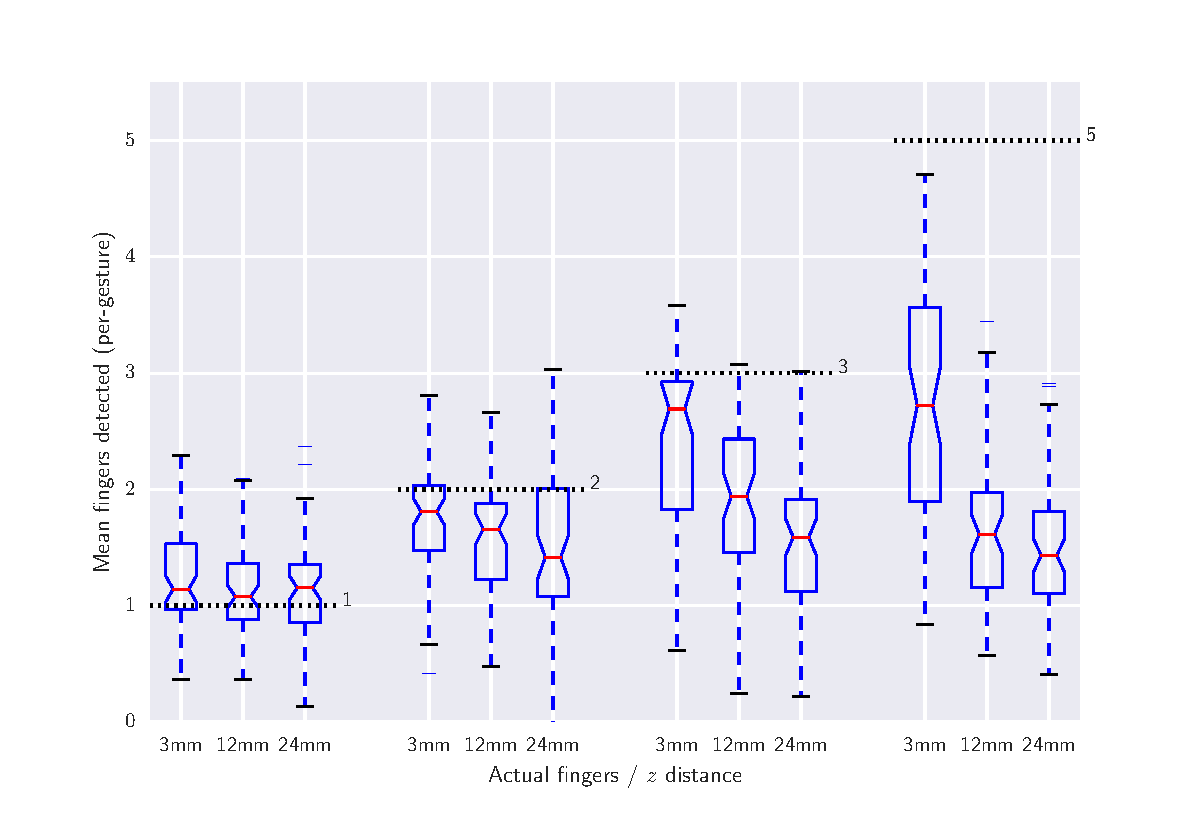
\includegraphics[width=1.0\linewidth]{images/boxplot_finger_distance.pdf}    

    \caption{Average number of fingers detected by the touch sensor at different heights above the surface, averaged over all gestures. Dashed lines indicate
    the true number of fingers present. The Box plots include bootstrapped uncertainty notches for the median. It is clear that the device is biased toward 
    undercounting fingers, particularly at higher $z$ distances.
    }

    % use the notation fig:name to cross reference a figure
    \label{fig:boxplot} 
\end{figure}


%==================================================================================================================================
\chapter{Conclusion}    
Summarise the whole project for a lazy reader who didn't read the rest (e.g. a prize-awarding committee). This chapter should be short in most dissertations; maybe one to three pages.
\section{Guidance}
\begin{itemize}
    \item
        Summarise briefly and fairly.
    \item
        You should be addressing the general problem you introduced in the
        Introduction.        
    \item
        Include summary of concrete results (``the new compiler ran 2x
        faster'')
    \item
        Indicate what future work could be done, but remember: \textbf{you
        won't get credit for things you haven't done}.
\end{itemize}

\section{Summary}
Summarise what you did; answer the general questions you asked in the introduction. What did you achieve? Briefly describe what was built and summarise the evaluation results.

\section{Reflection}
Discuss what went well and what didn't and how you would do things differently if you did this project again.

\section{Future work}
Discuss what you would do if you could take this further -- where would the interesting directions to go next be? (e.g. you got another year to work on it, or you started a company to work on this, or you pursued a PhD on this topic)

%==================================================================================================================================
%
% 
%==================================================================================================================================
%  APPENDICES  

\begin{appendices}

\chapter{Appendices}

Use separate appendix chapters for groups of ancillary material that support your dissertation. 
Typical inclusions in the appendices are:

\begin{itemize}
\item
  Copies of ethics approvals (you must include these if you needed to get them)
\item
  Copies of questionnaires etc. used to gather data from subjects. Don't include
  voluminous data logs; instead submit these electronically alongside your source code.
\item
  Extensive tables or figures that are too bulky to fit in the main body of
  the report, particularly ones that are repetitive and summarised in the body.
\item Outline of the source code (e.g. directory structure), 
    or other architecture documentation like class diagrams.
\item User manuals, and any guides to starting/running the software. 
Your equivalent of \texttt{readme.md} should be included.

\end{itemize}

\textbf{Don't include your source code in the appendices}. It will be
submitted separately.



\end{appendices}

%==================================================================================================================================
%   BIBLIOGRAPHY   

% The bibliography style is agsm (Harvard)
% The bibliography always appears last, after the appendices.

\bibliographystyle{agsm}

% Force the bibliography not to be numbered
\renewcommand{\thechapter}{0} 
\bibliography{l4proj}

\end{document}
